\documentclass[11pt]{article}

\usepackage{a4}
\usepackage{graphicx,color,psfrag}
\usepackage{amsmath,amssymb} 
\usepackage{multirow}
\usepackage{geometry}
\usepackage{xspace}
%\usepackage{../../../Latex_Packages/macros2}
%\usepackage[authoryear, sort, square]{natbib}
\usepackage[table]{xcolor}
\usepackage{macros}
\usepackage{mathrsfs}
\usepackage[numbers, sort, square]{natbib}
\usepackage{tabularx}

\usepackage{url}


\usepackage{fancyhdr}

\definecolor{greenGraph}{rgb}{0, 0.6, 0}

\setlength{\textheight}{25cm} 
\setlength{\topmargin}{-1.75cm}   
\setlength{\textwidth}{18cm}  
\setlength{\oddsidemargin}{-1cm} 
\setlength{\evensidemargin}{-1cm}

%\setlength{\oddsidemargin}{-5mm}	
%\setlength{\evensidemargin}{-5mm}
%\setlength{\topmargin}{-18mm}	
%\setlength{\parindent}{0mm}
%\setlength{\parskip}{1mm}
%\setlength{\textwidth}{170mm}
%\setlength{\textheight}{255mm}
%\setlength{\unitlength}{1mm}

\pagestyle{fancy}

\lhead{\nouppercase{\leftmark}} 
\chead{}
\rhead{\thepage}
\lfoot{}
\cfoot{}
\rfoot{}

\usepackage{setspace}  
\doublespacing

\title{Additional Notes on Creating Real Data for Testing and Validating 3D Reconstruction Methods from David 3D Scanner}

\author{
%{\bf Mathias Gallardo} \hspace{1cm} {\bf Toby Collins} \hspace{1cm} {\bf Adrien Bartoli} \\
~\\
EnCoV, IP, UMR 6602 CNRS, Universit\'e Clermont Auvergne / SIGMA, France \\
~\\
Corresponding author: Mathias Gallardo\\
{\tt Mathias.Gallardo@gmail.com}\\
~\\
}

\begin{document}

\maketitle
\thispagestyle{empty}

Most of methods developed in EnCoV deal with 3D reconstruction and require 3D ground-truth shape to test and validate them.
This document gives additional information about how to use the commercial structured light scanner from David 3D Scanner to reconstruct in 3D the shape of an object and to capture its texture.
A good tutorial provided by David 3D Scanner can be found in the attached folder ``docs'' and some Matlab codes in the attached folder ``codes''.

\textit{Prerequisites:}
These additional information are done for Windows.
We did not verify if it works for Linux or Mac.
In this document, we refer to this tutorial when using the notation p.X with X a page number of the tutorial.

\newpage
\tableofcontents
\newpage

\section{Overview}
The construction of ground-truth 3D datasets with the David 3D Scanner system requires four steps, which are illustrated in figure~\ref{fig:overview}.
For each step, we give some advices and solutions to problems we faced.

 \begin{figure}[h]
 	\begin{center}
 		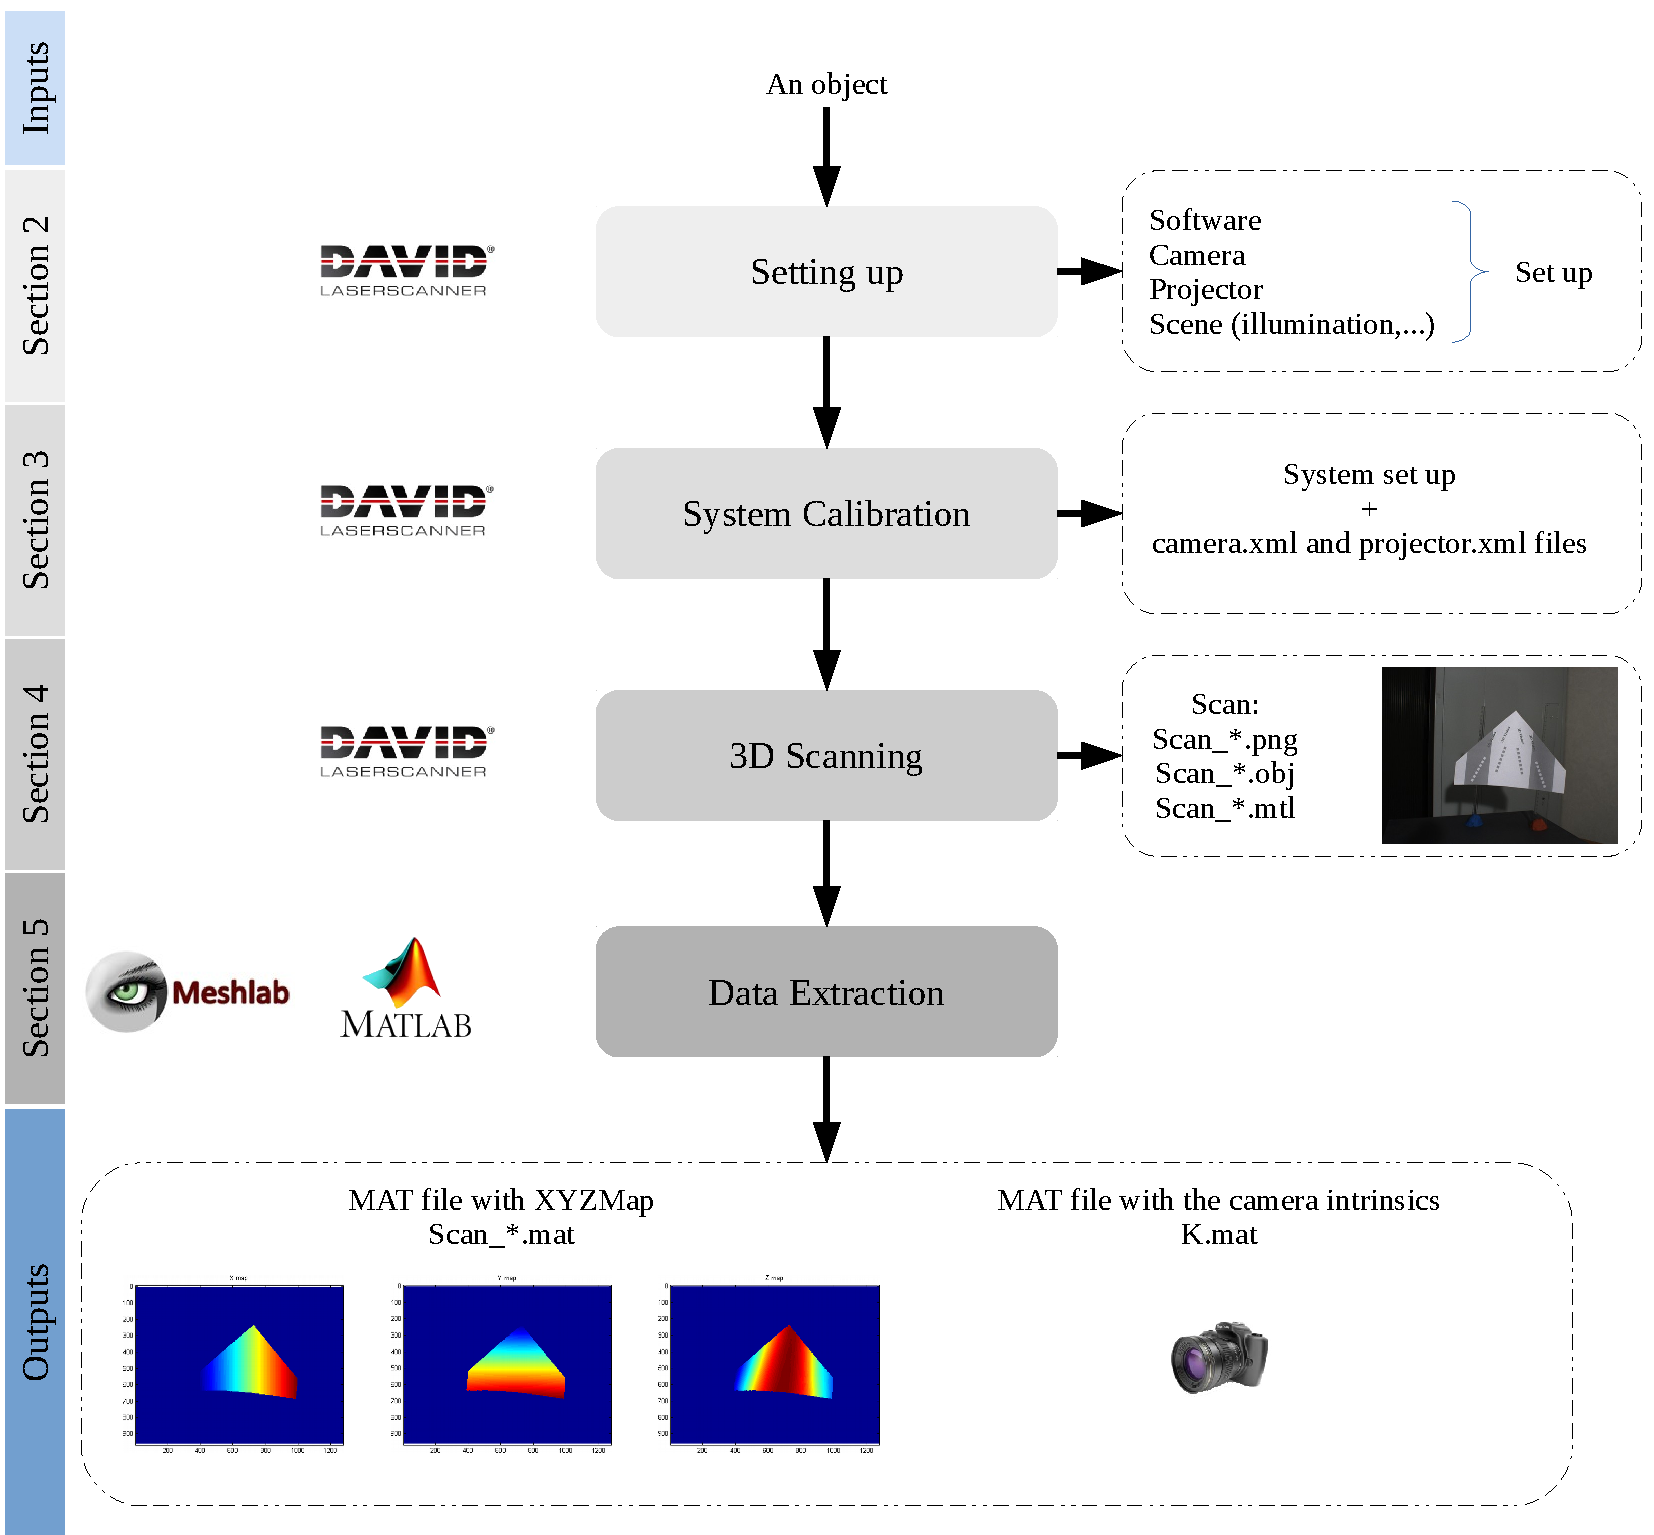
\includegraphics[width=15 cm]{images/overview.pdf}
 	\end{center}
 	\caption{Summary of the construction process of ground-truth 3D datasets with the David 3D Scanner system.}
 	\label{fig:overview}
 \end{figure}
\newpage

\section{Setting Up}
We first show how to set up the 3D Scanner system and the scene.
\subsection{David 3D Software Setup}
\subsubsection{Description}
The David software can be downloaded from the company website.
Once downloaded and installed, the pen driver shown in figure~\ref{fig:penDriver} has to be plugged into the computer to be permitted to use the software.
This pen driver contains the licence, which is not free.

\begin{figure}[h]
\begin{center}
 		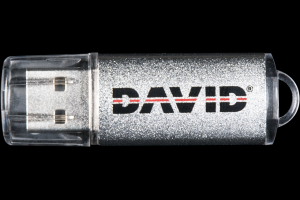
\includegraphics[width=6 cm]{images/licence.png}
 	\end{center}
 	\caption{The pen driver containing the David 3D licence.}
 	\label{fig:penDriver}
\end{figure}

\subsubsection{Which software version?}
If you plan to use the turntable, make sure running the 64 bits version of David 4 or newer versions.

\subsubsection{Possible Problems with the David 3D Software}
\subsubsection{David licence got corrupted}
The pen driver contains the licence which enables us to use David 3 and David 4.
A picture of this pen driver is given in figure~\ref{fig:penDriver}.
However, it could happen that the licence get corrupted.
The obtained error is the following:
\begin{verbatim}
licence status: non-negative number required
Parameter name: count.
You won't be able to save in Shapefusion, and new scans can only be saved in a reduced resolution
\end{verbatim}

To solve this licence problem, there are several solutions to test in the following order:
\begin{enumerate}
\item use another USB plug
\item reboot the computer
\item use another computer
\item download the installer of the David software and during the installation process, use the option ``Update original DAVID USB flash drive'' 
\item the last solution is to send a message to { \tt info@david-3d.com}.
Explain all the steps you went through and ask them if they can check if the licence got corrupted.
If the answer is positive, you will have to send the RegID and the .lic file and then the company support will send you a new licence.
\end{enumerate}

\paragraph{How to get the RegID?}
We can find it in the terminal which appears while opening the software.
However, this terminal closes immediately after and, even if you thick the option to not close it (``David Software $\rightarrow$ Settings $\rightarrow$...''), you can not copy-paste the RegID.
To avoid this problem:
\begin{itemize}
\item open a terminal
\item change the directory to the folder where the {\tt .exe} is
\item execute the following command line: {\tt david4\_x64.exe $>$ log.txt}
\end{itemize}
This command writes in a .txt file the text displayed in the terminal.

\subsubsection{Cannot find the projector with David 5}

\paragraph{Problem.}
The David 5 software does not propose you any projector in the ``Setup'' menu in the GUI.

\paragraph{Solution.}
Before going further, here a list of solutions which can be used to identify the problem.
If none of these solutions work, move to the next paragraph.
\begin{itemize}
\item switch the output plugs for the main screen and the projector
\item extend the screen
\item try with another type of projector of the same company
\end{itemize}

A possible cause of this problem is TeamViewer, if it is installed.
To be sure about the cause of the problem, have a look at the ``Device manager'' window and if you notice that the projector is associated to TeamViewer, then uninstalling TeamViewer is the correct solution.
The reason is that, once installed, TeamViewer changes the configuration of the monitor.
Even if you uninstall TeamViewer, the problem remains.
One solution is the following:
\begin{enumerate}
\item go to ``Device Manage''
\item click right on the ``Monitor PnP -...''
\item click left on ``Uninstall''
\item click right on ``Monitors''
\item click left on ``Scan for hardware changes''
\end{enumerate}
The projector will appear with a name close to ``Generic monitor...'' and now you can select the projector on the David 5 software.


\subsection{Camera Setup}
Before using the David software, we have to setup the camera.
In the lab, we use cameras from Point Grey (now FLIR).
To use these cameras:
\begin{itemize}
\item go to \url{https://www.ptgrey.com/support/downloads}
\item create an account
\item select the ``Product Families'', the ``Camera Models'' and then the ``Operating System''
\item then, download and enable all options:
\begin{itemize}
\item the SDK
\item the GTK runtime
\item the Viewer
\end{itemize}
\end{itemize}

\subsection{Scene Setup}
\begin{enumerate}
\item before setting the projector and the camera, one has to define the place where to place the object.
For this, one main rule is the following: 

\noindent
\fbox{\begin{minipage}{\linewidth}
The object has to be fully lit by the projected calibration pattern and that the lit regions of the object has to be visible from the camera
\end{minipage}}

\item a support, such as plastic box or books (avoid reflective surfaces), can be used to put the object at the correct height
This setup is important because camera and projector configurations depend on the scene height and the object size.
\item if possible, turn off all the room lights. Some artifical light sources can flicker, which forces the camera to change automatically its parameters
\item if you plan to use the turntable, make sure that the object is stable to rotation and most of the desired parts are visible.
\end{enumerate}

\subsubsection{Coarse setup of the camera and the projector}
\begin{enumerate}
\item you can try different angles (between the camera optical axis and the projector optical axis) in the range of $15^{\circ}$ to $40^{\circ}$
\item camera and projector have to be at the same height
\item make sure that the camera and the projector are physically stable. 
A small displacement of the camera or the projector requires to perform again the system calibration, given in~\S\ref{sec:systemCalib}.
\item projector setup:
\begin{itemize}
\item after turning on the projector, in the tab ``Setup'' of the software GUI, the screen ID has to be set up at ``2'' to provide the good input to the projector
If you are in the ``Calibration'' tab, you will see the calibration cardboard from the camera stream
\item the distance between the projector and the object depends on the size of the object.
The section ``Working distance'' p.3 gives good advice to set this distance.
\item look at the sharpness of the projected calibration pattern and adjust the zoom and the focal length of the projector directly on the projector
\end{itemize}
\item camera setup:
\begin{itemize}
\item put the camera closer to the scene such that the focus is good
\item orientate the camera such that:
\begin{itemize}
\item the object is in the middle of the camera image
\item the six circles of the calibration cardboard, shown in figure~\ref{fig:calibCardboard} with the orange circles, are visible and well distributed around the middle of the camera image.
\end{itemize}
\end{itemize}

 \begin{figure}[h]
 	\begin{center}
 		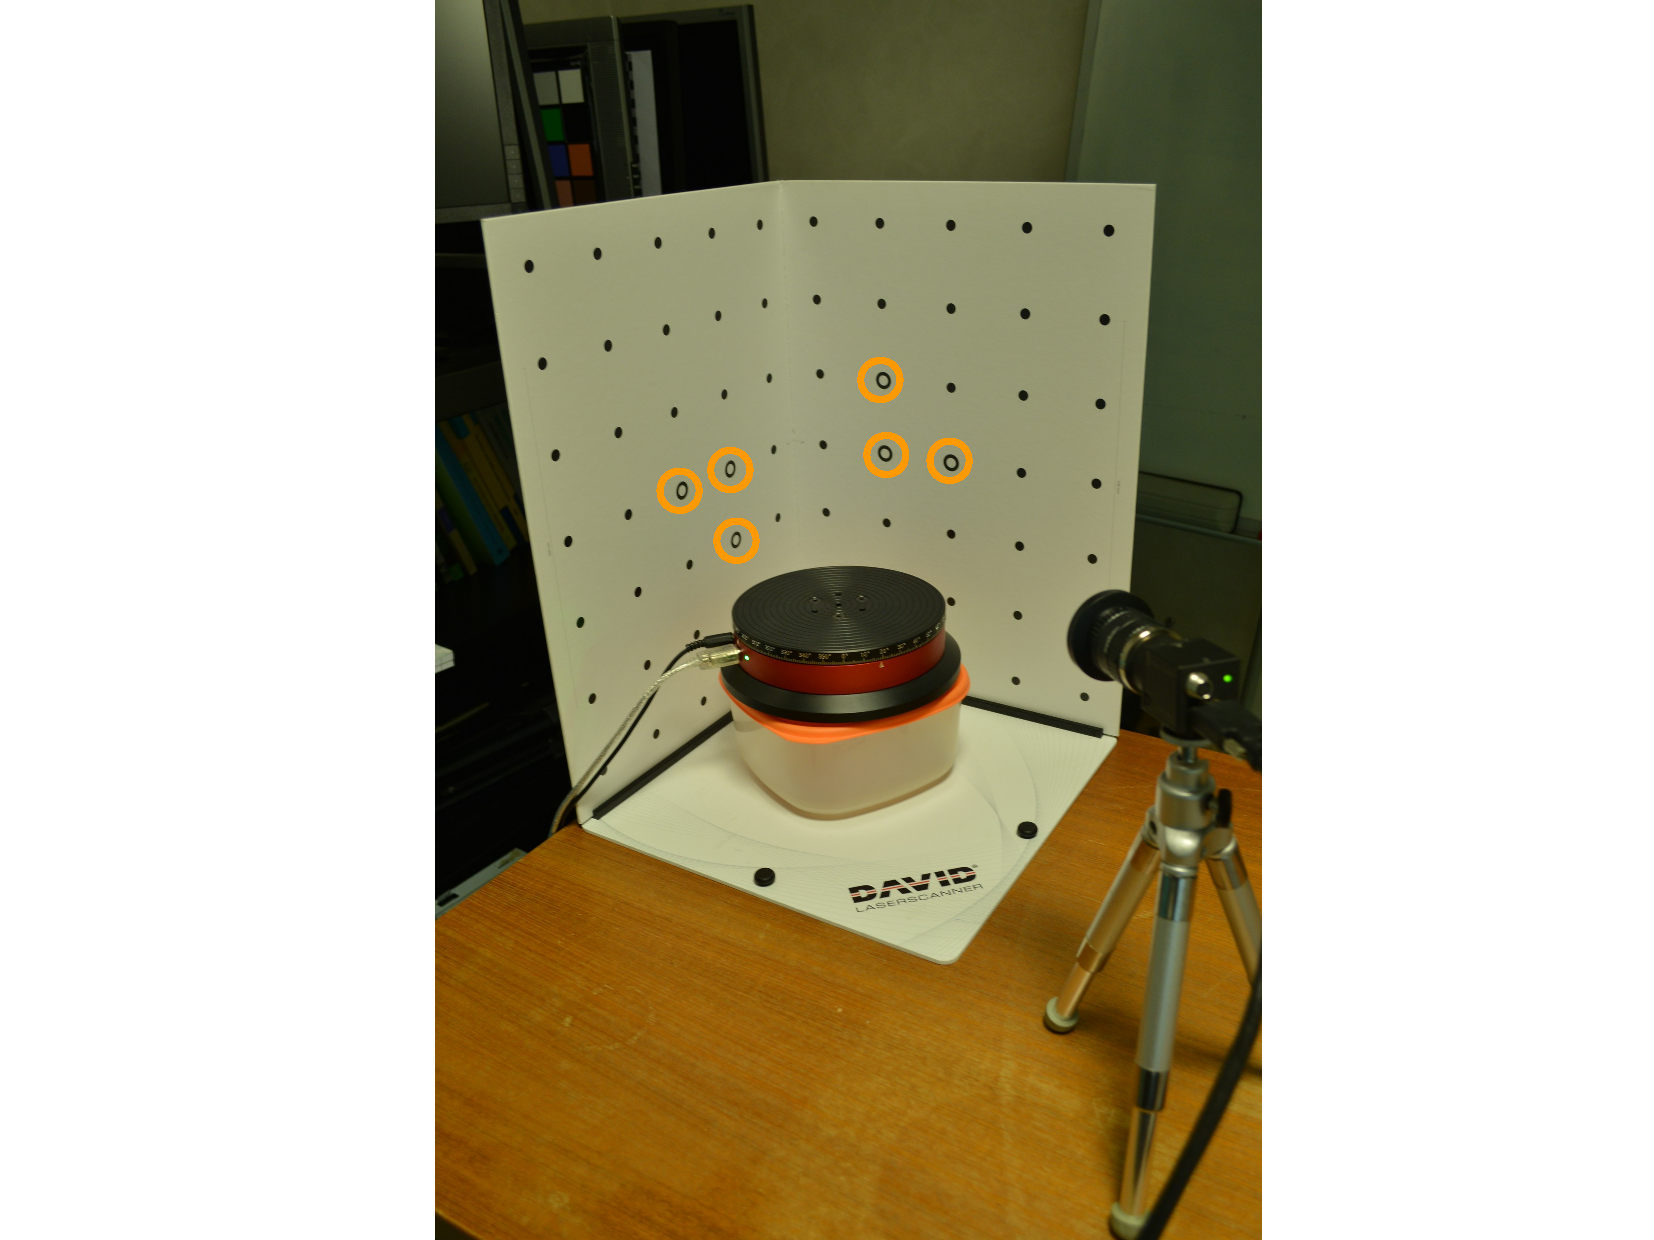
\includegraphics[width=11 cm]{images/calibCardboard.pdf}
 	\end{center}
 	\caption{The calibration cardboard.}
 	\label{fig:calibCardboard}
 \end{figure}

\item the camera parameters have to be fixed physically:
\begin{itemize}
\item Type of images: YUV/RGB, 8 bits, 24 bits,...? This is an important choice if you want to grab texture at the same time. If yes, select RGB 8 bits
\item Focal length: can be fixed directly on the camera. Take a look at ``Camera focus'' section (p.4)
\item Gain: can be fixed in the David GUI: set it at 0 if possible
\item Fps: can be fixed in the David GUI: higher is better
\item Brightness/Aperture: can be fixed directly on the device. Take a look at ``Camera brightness / aperture'' section (p.4)
\item Exposure: can be fixed in the David GUI. Take a look at ``Exposure time'' section (p.4)
\item Shutter: can be fixed in the David GUI. This parameter has a strong impact on the image quality and on the surface texture.
\end{itemize}
\item now, the camera parameters have to be fixed physically:
\begin{itemize}
\item Type of images: YUV/RGB, 8 bits, 24 bits,...? This is an important choice if you want to grab texture at the same time. If yes, select RGB 8 bits
\item Focal length: can be fixed directly on the camera. Take a look at ``Camera focus'' section (p.4)
\item Gain: can be fixed in the David GUI: set it at 0 if possible
\item Fps: can be fixed in the David GUI: higher is better
\item Brightness/Aperture: can be fixed directly on the device. Take a look at ``Camera brightness / aperture'' section (p.4)
\item Exposure: can be fixed in the David GUI. Take a look at ``Exposure time'' section (p.4)
\item Shutter: can be fixed in the David GUI. This parameter has a strong impact on the image quality and on the surface texture.
\end{itemize}

\paragraph{Camera parameters automatically changing.}
Note that the camera parameters can be automatically changed by the David software.
This can be undesirable in the case where you plan to use pixel intensities.
To fiw the camera parameters, go to ``Settings $\rightarrow$ Advanced Settings $\rightarrow$ Camera'' and disable ``EnableAutoPropertyHandling'' and ``EnablePhysicalExposureMapping''.

\paragraph{Irradiance images.} Setting the image format at YUV and the gamma value at 1 provides images which can be considered as irradiance images.
\end{enumerate}

\section{System Calibration}
\label{sec:systemCalib}
\subsection{Some Advices for the System Calibration}
\begin{enumerate}
\item put the selected calibration cardboard shown in figure~\ref{fig:calibCardboard}.
The calibration cardboard has to be placed at the middle of the object (which is then removed for this step)
\item find the scale number (in the border of the calibration cardboard) and correct the scale in the ``Calibration'' GUI area
The object and the space defined by the six circles in the calibration cardboard must have the same size.
Two calibration cardboards, with four different sizes, are available in the lab.
The number (the calibration scale) associated to the selected calibration cardboard is the one to provide in the tab ``Calibration''
\item check again if the six circles are in the middle of the camera image (Cf. p.8 ``Check camera image'')
\item select ``both'' for the ``Calibration -> Orientation''
\item run the ``Calibration'' process
\item if calibration works, go to ``Scanning'' tab, select ``default'' as type of scanning and scan the calibration cardboard
\item if the obtained 3D scan is dense enough (\textit{i.e.} without big holes), we can consider that the calibration of the setup is good.
\end{enumerate}

This step is equivalent to a fine setup of the projector and the camera.
For all the other steps, the attached tutorial provides all information.

\subsection{Possible Problems with the System Calibration}
If the calibration does not work or if it is not good enough, try the following scene changes:
\begin{itemize}
\item change the angle between the camera and the projector
\item change the height of the projector and the camera
\item change the position and the orientation of the calibration cardboard
\item change the camera properties: lower gain (around 0 dB) or the exposure
\item change the projector properties: brightness, in both directions (darker or brighter)
\end{itemize}

\section{3D Scanning with the David 3D Scanner}
The scanner system can be used to scan a surface or a volume.
Both processes are well explained in the tutorial provided by the company and given in the folder ``docs''.
We then give here some remarks about problems we faced and the tips we found while scanning a surface or a volume.

\subsection{Possible Problems with the Surface Scanning}
\subsubsection{Background removal}
This option can be very useful because the obtained scans of the object of interest require less cleaning.
This option is also necessary while enabling the auto-alignment of scanning using the turntable or not.
Note that, while using the turntable, the David software tries to match also the 3D points in the background, which may lead to incorrect registration.

\subsubsection{Limitation with black regions}
As the scanner uses structured-light, black surfaces may not be recovered.
This is visible in figure~\ref{fig:blackRegions}.
We provide here two solutions:
\begin{itemize}
\item scan the object from different viewpoints
\item change the brightness of the projector
\end{itemize}

 \begin{figure}[h]
 	\begin{center}
 		
\includegraphics[width=15 cm]{images/illustration_blackregions.png}
 	\end{center}
 	\caption{Left: the mesh of a reconstructed piece of t-shirt, where we can observe some holes. Right: the texture-map mesh of the same object.}
 	\label{fig:blackRegions}
 \end{figure}
 
\subsubsection{Bad scans}
Some scans can be less dense. Two solutions are:
\begin{itemize}
\item increase the brightness of the projector
\item perform the scanning process with a higher quality.
\end{itemize}

\subsubsection{Texturing}
This tab shows you the camera image which will be used to texture-map the 3D scan.
Note that the scanning procedure will automatically take the texture-map (if the associated option is enabled), but, in some cases, you may want to have a texture-map acquired in different illumination conditions.
To do so, after each scan:
\begin{itemize}
\item go to the ``Texturing'' tab
\item fiw the scene illumination (turning on additional light sources,...)
\item grab the new texture
\item check in the ``3D Shape'' tab the new texture. Note that grabbing a new texture creates in the ``3D Shape'' tab a new scan.
\end{itemize} 

\subsubsection{Scanning a complex object}
This can be done with this system under some conditions.
Usually, to scan completely an object, we need to scan it from different viewpoints, move the object to scan the hidden surfaces and then register them to the scans of the first sequence.
For instance, in the case of cube, we can use the turntable and then, we have to move the cube under the turntable to scan the face which was not visible in the first sequence of scans.

If the object is rigid, the scanning limitation is set by the angle between the projector and the camera.
Indeed, to be reconstructed, a surface region has to be lit by the pattern and seen by the camera, which can be very difficult or even impossible in some cases.

If the object is deformable, the scanning limitation is set by the fact that the object shape will change when, after a first sequence of scans, we will move it to scan the hidden surfaces.
In the lab, this was the case of the silicon liver we tried to scan.
This is difficult since using the turntable the camera does not allow the scanner system to see the whole surface, which makes that usually the bottom part is missing.
From this problem, we thought about two ideas which circumvent this difficult.

\paragraph{Solution 1: scanning the object in two positions}
We determine in advance the two positions of the object such that each region of the object surface is visible in at least one of the two sequences of scans \emph{and} such that the object shape is preserved between the two sequences.
Any type of support can be used to make the position stable.
Note that the support can be removed manually from the scan.

\paragraph{Solution 2: using two cameras (not tried)}

Since David 5, we can use simultaneously two cameras.
This can be very interesting for deformable objects, but this has to be tested.

\subsection{Possible Problems with the Volume Scanning}
\subsubsection{Difficult registration of multiple scans}
Manual and automatic registration of multiple scans can be a very difficult task.
This comes from the fact that, in both types, the registration tries to fit the shape and/or the texture of a small region of two scans.
This process can be made easier while using the turntable using the following tip: scanning a little region of the top of the turntable .
This can work because, as at the top of the turntable, the shape of two successive scans is the same, but it is not the case for the texture which is also very discriminative at these regions.

\subsubsection{Wrong texture in my scan}
This problem is illustrated by figure~\ref{fig:wrongTexture}(a).

\begin{figure}[h]
\begin{center}
 		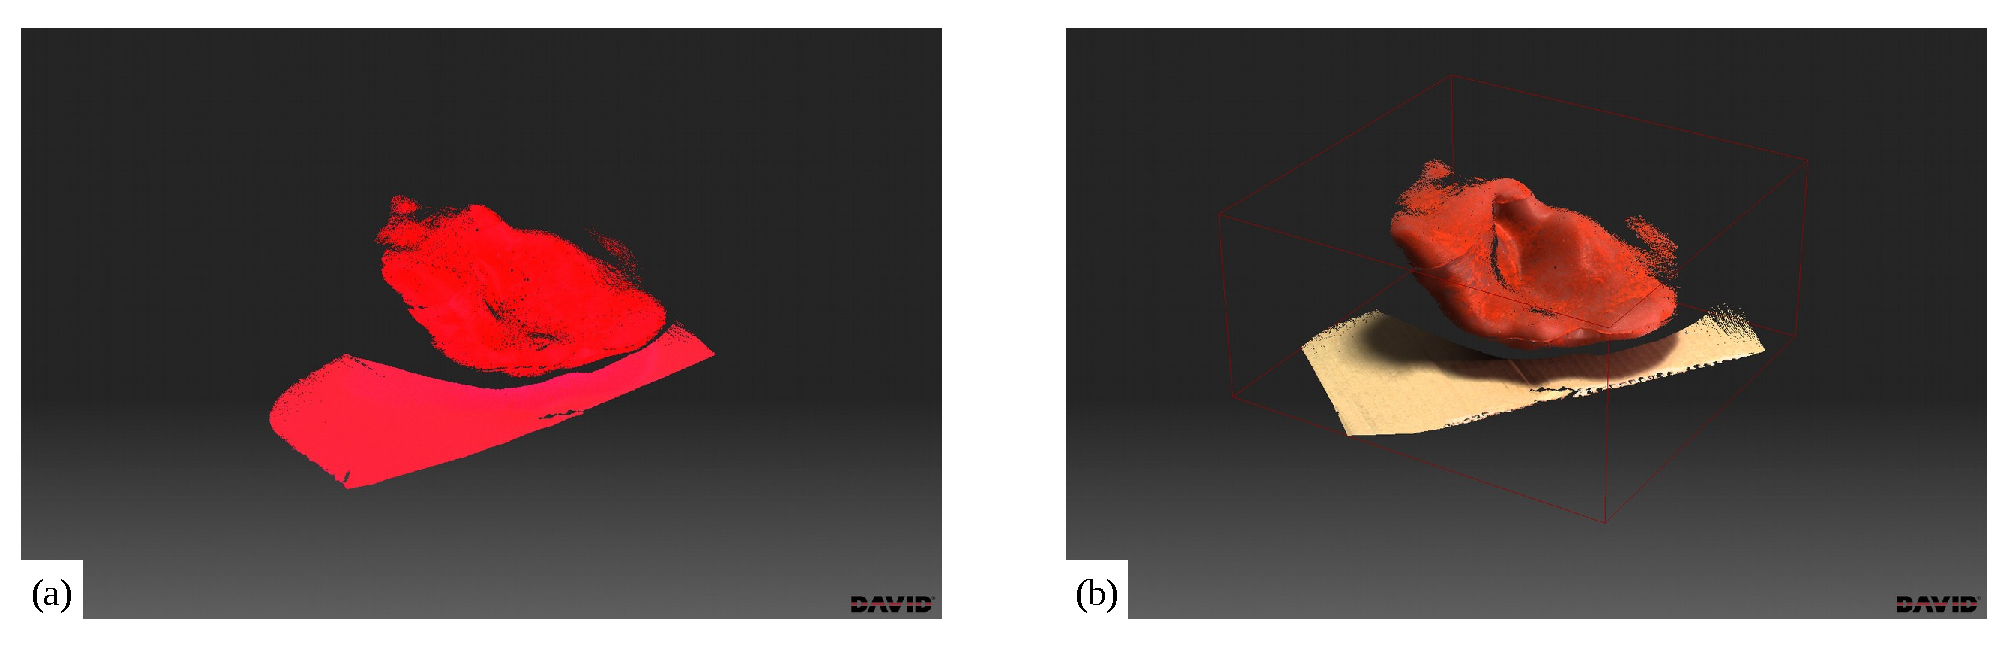
\includegraphics[width=15 cm]{images/illustration_wrongTexture.pdf}
 	\end{center}
 	\caption{(a) Scan with wrong texture. (b) Scan with real texture.}
 	\label{fig:wrongTexture}
\end{figure}

One important point to note is that the video flow gives a good natural image of the scene in the tab ``Scanning'' and ``Texturing'' of the GUI.
The 3D scanning works well, but the texture grabs is wrong and looks saturated.
The solution to this problem is to perform a ``White Balance Correction''.
To do this, scan a white large object, such as the back of the calibration pattern and then click on ``White Balance Correction''.
A result is provided in figure~\ref{fig:wrongTexture}(b).

\subsubsection{Wrong texture after fusion}
After fusing two scans, one can obtain a wrong texture, \eg a brown texture in figure~\ref{fig:brownTexture}(d).
That happens when you try to fuse two fusion results, given by figures~\ref{fig:brownTexture}(a) and~\ref{fig:brownTexture}(b).
Note that only scans can be fused and not fusion results.

\begin{figure}[h]
\begin{center}
 		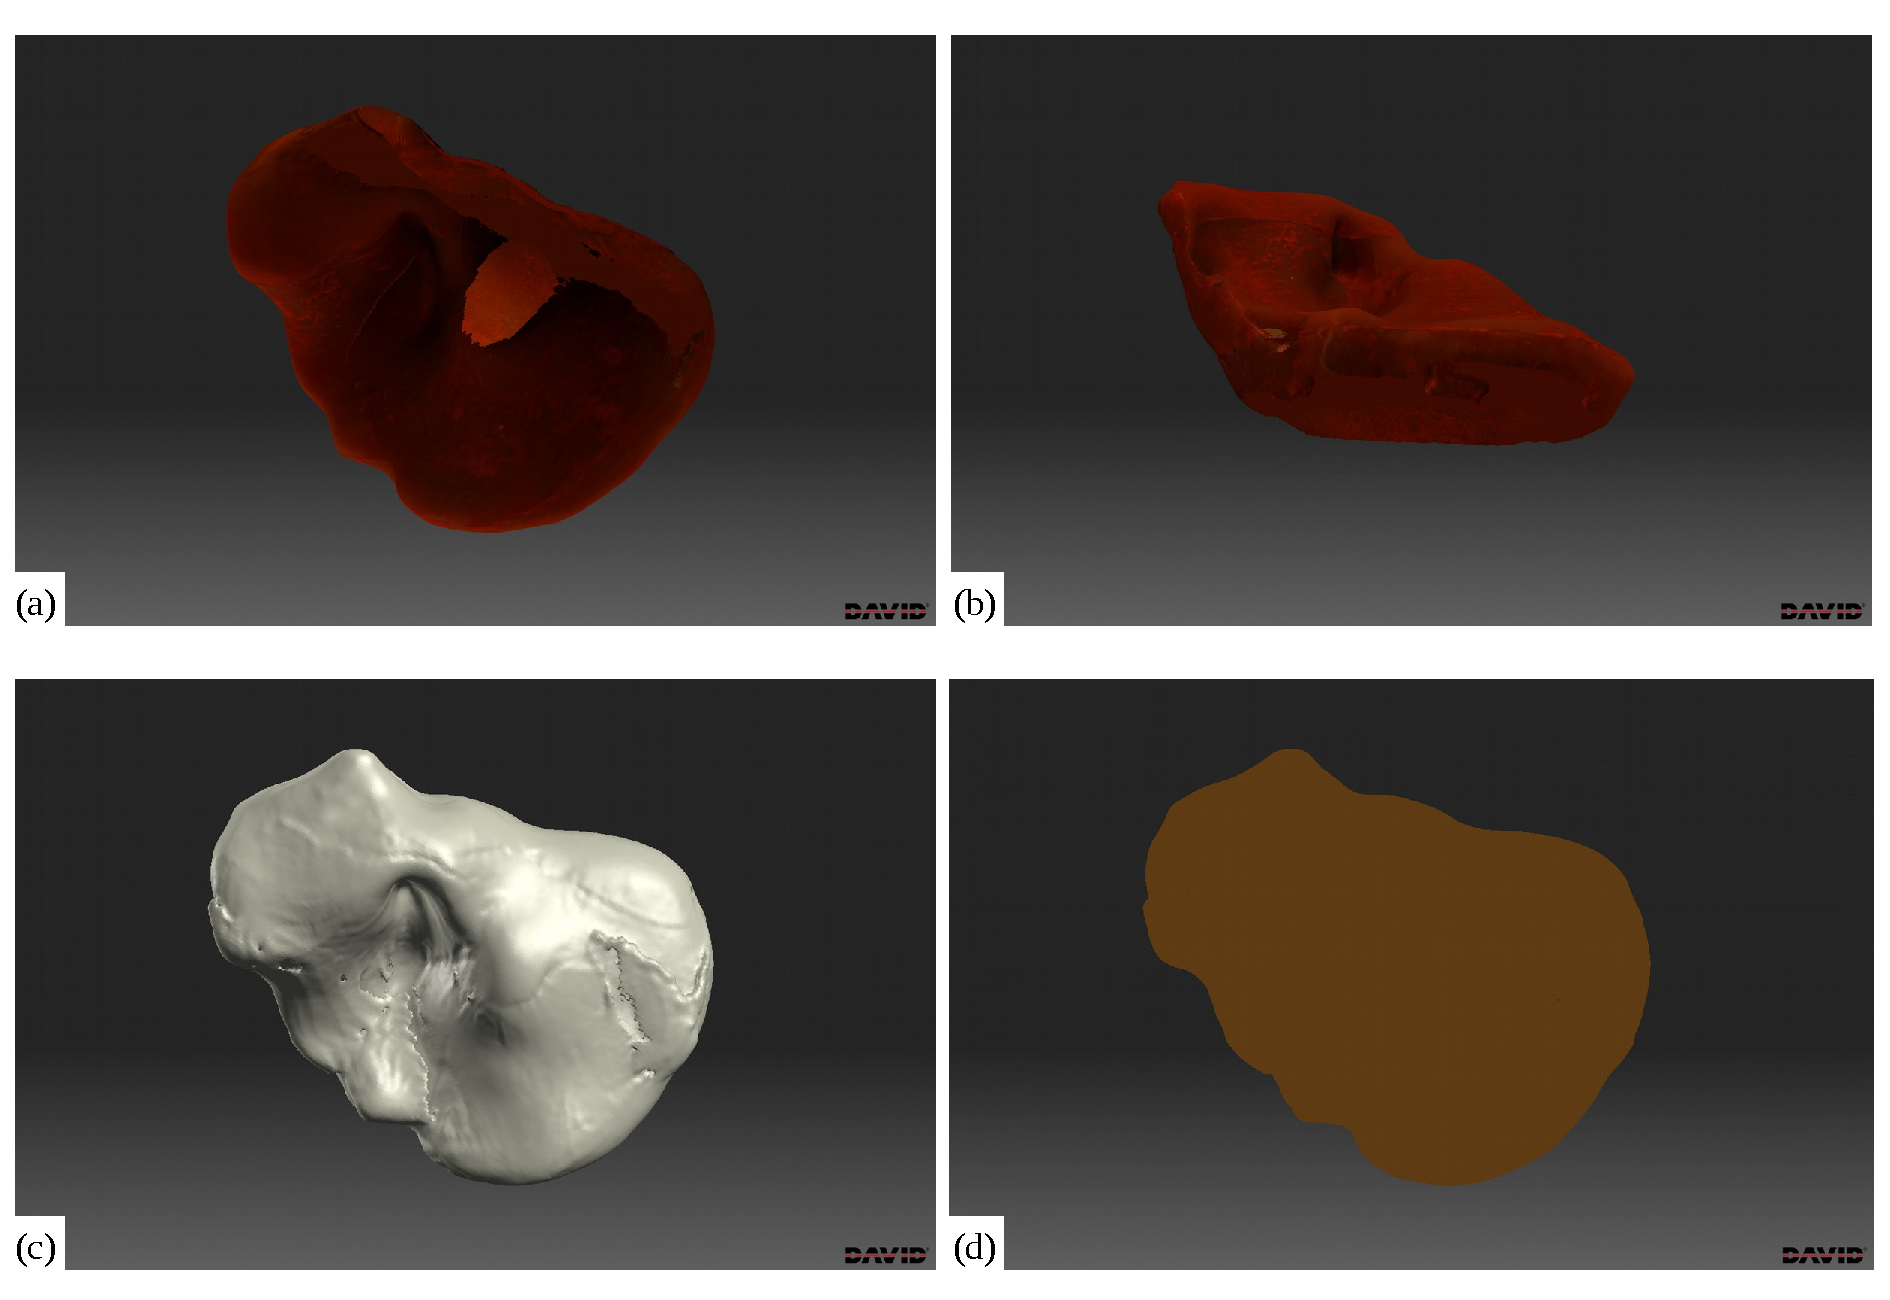
\includegraphics[width=15 cm]{images/illustration_brownTexture.pdf}
 	\end{center}
 	\caption{(a) Fusion result of the bottom part of the silicon liver. (b) Fusion result of the top part of the silicon liver. (c) Shape obtained by fusing the fusion results of (a) and (b). (d) Shape and texture obtained by fusing the fusion results of (a) and (b). We can note that the texture is wrong.}
 	\label{fig:brownTexture}
\end{figure}

Several ways to prepare a shape fusion are proposed at the following link:
\url{http://wiki.david-3d.com/david3_user_manual/shape_fusion}

One good solution is to use the option ``Contact Pair Selection'':
\begin{enumerate}
\item put a thick in the ``Contact Pair Selection'' box
\item click on ``Align Scans''
\item search for a remarkable point present in both surfaces
\item click on the remarkable point on the surface you want to move
\item double click on the remarkable point on the surface you want to reconstruct and wait
\end{enumerate}

Then, you can go to step 13 described in the previous link and perform a ``Global Fine Registration'' and a shape fusion.


\section{Data Extraction with MeshLab and Matlab}
\subsection{Mesh Processing with MeshLab}

Meshes constructed by the David 3D Scanner have to be cleaned and decimated in order to have ground-truth datasets which are proper, easy-to-use and fast to load and manipulate.
Before extracting the data on Matlab, here a list of processings that have to be done under MeshLab:
\begin{enumerate}
\item decimate the mesh to $10,000$ faces using ``Remeshing, Simplification and Reconstruction $\rightarrow$ Quadratic Edge Collapse Decimation (with texture)''
\begin{itemize}
\item Target number of faces: $10,000$
\item Preserve boundary of the mesh: disabled
\item Optimal position of simplified vertices: enabled
\item Preserve Normal: disabled
\item Planar Simplification: disabled
\item Simplify only selected faces: disabled
\end{itemize}
\item click on ``Cleaning and Repairing $\rightarrow$ Remove Faces from Non Manifold Edges''
\item click on ``Fill Holes'' in the toolbar and select the holes to be filled
\item click on ``Smoothing, Fairing and Deformation $\rightarrow$ Laplacian smooth (surface preserve)'': iterate such that the surface ids smooth enough
\item click on ``Cleaning and Repairing $\rightarrow$ Compact faces''
\item click ``File $\rightarrow$ Export Mesh As...'', select the \texttt{.obj} format and disable every option \emph{except} ``Wedge $\rightarrow$ TexCoord''. Three files will be created: the material file \texttt{.mtl}, the 3D mesh \texttt{.obj} and the texture-map \texttt{.png}.
\item open the \texttt{.mtl} file and remove all the materials without \texttt{map\_Kd}. A new material is defined by a paragraph starting by \texttt{newmtl}.
\end{enumerate}


\subsection{Data Formatting with Matlab}

The folder ``codes'' contains two codes to prepare 3D scans for validation of 3D reconstruction methods:
\begin{itemize}
\item {\tt readDavidScannerCamFile.m}: reads the intrinsic and extrinsic parameters of the camera from the camera calibration file provided by the David 3D Scanner software (after the step of camera calibration)
\item {\tt main\_computingXYZMap\_DavidScanner.m}: shows how to read the 3D mesh created by David 3D Scanner and computes and saves the XYZ map of the scan.
\end{itemize}

The required libraries are provided in the subfolder ``toolboxes''.



\end{document}



